% figure: 高数-单位圆三角不等式.png
% 用途：高数《附录 三角与代数补充》—— 单位圆面积夹逼证明 sin x < x < tan x
% 构建：..\build.ps1 -File .\trig-inequality-unit-circle.tex
% 几何：单位圆半径 4cm，取 x = 50°；M=(cos x, 0) 为 B 在 x 轴的投影，T=(1, tan x) 是
%       过 A 的切线与射线 OB 的交点。三角形 OAB ⊂ 扇形 OAB ⊂ 三角形 OAT，
%       三者面积依次为 ½sin x、½x、½tan x，两边同乘 2 即得结论。
% 注意：\R 或 \xa 改动后，T 的纵坐标、角弧与 B 处标签位置都会跟着变，无需另改。
\documentclass[border=10pt]{standalone}
\usepackage{fontspec}
\setmainfont{Cambria}
\usepackage{unicode-math}
\setmathfont{Cambria Math}
\usepackage{tikz}
\usetikzlibrary{calc}
\usepackage{amsmath}
\usepackage{ctex}

\definecolor{figink}{HTML}{1E2228}      % 图线主色
\definecolor{figacc}{HTML}{B23020}      % 强调色（角弧、结论式）
\definecolor{figfill}{HTML}{EDF2F9}     % 三角形 OAT 填充（浅）
\definecolor{figsector}{HTML}{D7E3F4}   % 扇形 OAB 填充（深一档）
\definecolor{figsub}{HTML}{606874}      % 次要参考轴

\begin{document}
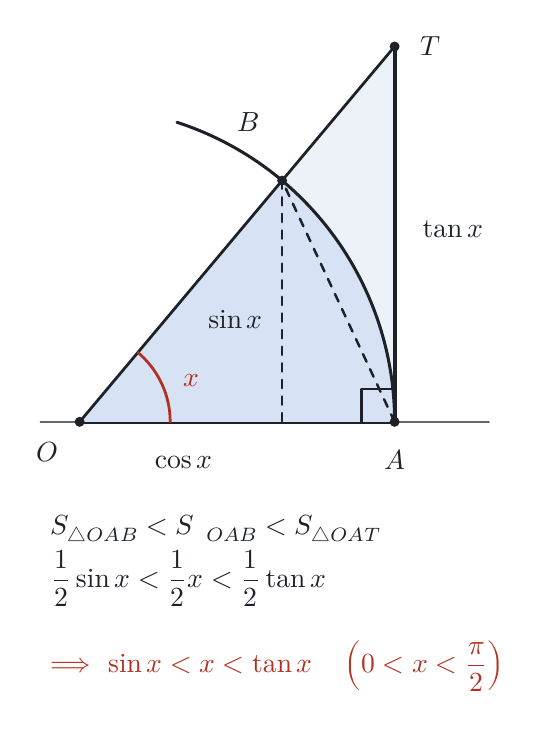
\begin{tikzpicture}[x=1cm, y=1cm, line width=1.0pt, line cap=round, line join=round]
  \def\R{4}
  \def\xa{50}
  \coordinate (O) at (0,0);
  \coordinate (A) at (\R,0);
  \coordinate (B) at (\xa:\R);
  \coordinate (M) at ({\R*cos(\xa)},0);
  \coordinate (T) at (\R,{\R*tan(\xa)});

  % 参考轴（次要）：只留 x 轴，它同时是三角形 OAB / OAT 的底边
  \draw[figsub, line width=0.5pt] (-0.5,0) -- (5.2,0);
  \draw[figink, line width=1.2pt] (O) -- (A);

  % 两个嵌套区域：先铺三角形 OAT，再在它上面铺扇形 OAB
  \fill[figfill] (O) -- (A) -- (T) -- cycle;
  \fill[figsector] (O) -- (A) arc (0:\xa:\R) -- cycle;

  % 圆弧（越过 B 一点，示意这是整段单位圆）
  \draw[figink, line width=1.1pt] (\R,0) arc (0:72:\R);

  % 半径 OT（B 在其上）与切线 AT（即 tan x）
  \draw[figink] (O) -- (T);
  \draw[figink, line width=1.4pt] (A) -- (T);
  % 弦 AB 与垂线 BM（即 sin x），虚线
  \draw[figink, line width=0.9pt, dashed] (A) -- (B);
  \draw[figink, line width=0.9pt, dashed] (B) -- (M);

  % A 处直角标记
  \draw[figink, line width=0.8pt] ($(A)+(-0.42,0)$) -- ($(A)+(-0.42,0.42)$) -- ($(A)+(0,0.42)$);

  % 圆心角弧
  \draw[figacc, line width=1.0pt] (1.15,0) arc (0:\xa:1.15);
  \node[figacc] at (1.42,0.53) {$x$};

  % 顶点
  \foreach \p in {O,A,B,T} { \fill[figink] (\p) circle (1.8pt); }
  \node[figink, anchor=north east] at (-0.14,-0.12) {$O$};
  \node[figink, anchor=north]      at (4.00,-0.22)  {$A$};
  % B 的标签放圆外左上：射线 OT 在 x=2.7 处已到 y=3.24，标签框若贴射线会压线
  \node[figink, anchor=south east] at (2.40,3.55)   {$B$};
  \node[figink, anchor=west]       at (4.20,4.77)   {$T$};

  % 三条线段的名字（都落在空白处，不需要白底遮罩）
  \node[figink, anchor=east]   at (2.46,1.30)  {$\sin x$};
  \node[figink, anchor=north]  at (1.32,-0.30) {$\cos x$};
  \node[figink, anchor=west]   at (4.22,2.45)  {$\tan x$};

  % 结论（图下两行，贴着图放，避免整体过高）
  \node[figink, align=left, anchor=north west] at (-0.5,-1.05)
    {$S_{\triangle OAB}<S_{\text{扇形}\,OAB}<S_{\triangle OAT}$\\[2pt]
     $\dfrac{1}{2}\sin x<\dfrac{1}{2}x<\dfrac{1}{2}\tan x$};
  \node[figacc, align=left, anchor=north west] at (-0.5,-2.65)
    {$\Longrightarrow\ \sin x<x<\tan x\quad\left(0<x<\dfrac{\pi}{2}\right)$};
\end{tikzpicture}
\end{document}
